\chapter{Problèmes non stationnaires}\label{Ch-temps}
\begin{abstract}
Dans ce chapitre, nous nous intéresserons (brièvement) au cas non stationnaire. Toutefois, nous n'aborderons pas les EF espace-temps, car il s'agit d'une formulation gourmande en ressources, d'où sa très faible utilisation (bien que la méthode soit en elle-même intéressante).

Dans ce chapitre, nous aurons besoin de «dériver numériquement», i.e. de construire des schémas numériques approchant des dérivées. Le chapitre~\ref{Ch-ED} en annexe permettra à certains de se rafraîchir la mémoire en regardant comment on résout les équations différentielles et EDP directement... puis numériquement. Nous utiliserons en effet la méthode de Newmark\index[aut]{Newmark (Nathan Mortimore), 1910-1981, Américain} décrite au paragraphe~\ref{Sec-Newmark}.
\end{abstract}

\medskip
\section{Équation non stationnaire de la dynamique}\index{ED-EDP!relation fondamentale de la dynamique}

Considérons l'équation de la dynamique, sous forme non stationnaire (i.e. dépendant du temps):
\begin{equation} M \ddot u(t) + C \dot u(t) + K u(t)= F(t) \end{equation}
qui sous forme discrétisée par éléments finis sera réécrite:
\begin{equation} \MM{M}\VV{\ddot q}(t) + \MM{C}\VV{\dot q}(t) + \MM{K}\VV{q}(t)= \VV{F}(t) \end{equation}
avec les conditions initiales~$\VV{q}(t=0)=\VV{q}_0$ et~$\VV{\dot q}(t=0)=\VV{\dot q}_0$.

\medskip
On cherche à obtenir la discrétisation~$\VV{q}$ du champ~$u$ et ses dérivées temporelles~$\VV{\dot q}$ et~$\VV{\ddot q}$ à différents instants~$t$ et vérifiant l'équation de la dynamique.

\medskip
Pour résoudre un tel problème, on se propose de réaliser une \textcolorblue{discrétisation temporelle} qui pourra être explicite ou implicite.

\medskip
Le schéma généralement utilisé pour la discrétisation temporelle est celui de Newmark,\index[aut]{Newmark (Nathan Mortimore), 1910-1981, Américain} (qui est présenté dans le cas de la résolution des équations différentielles au paragraphe~\ref{Sec-Newmark}, ce complément nous ayant été demandé).
Le schéma le plus général est, $\Delta_t$ représentant le pas de temps:
\begin{equation}
\begin{aligned}
&\VV{q}_{t+\Delta_t} = \VV{q}_t + \Delta t \VV{\dot q}_t + \frac{\Delta_t^2}2\left((1-2\beta)\VV{\ddot q}_t
+2\beta\VV{\ddot q}_{t+\Delta_t}\right) \\
&\VV{\dot q}_{t+\Delta_t} = \VV{\dot q}_t+\Delta_t\left((1-\gamma)\VV{\ddot q}_t+\gamma\VV{\ddot q}_{t+\Delta_t}
\right)
\end{aligned}
\end{equation}
que nous avons écrit sous la forme discrétisée, mais qui serait valable pour l'approximation continue (comme présenté au chapitre au paragraphe~\ref{Sec-Newmark}).

Les différents \textcolorblue{schémas de Newmark}\index[aut]{Newmark (Nathan Mortimore), 1910-1981, Américain} correspondent à des valeurs particulières de~$\beta$ et~$\gamma$.



\bigskip
\section{Schéma explicite: différences finies centrées}\index{schéma! des différences finies centrées}

Dans le cas \textcolorred{$\beta=0$ et~$\gamma=1/2$}, on retombe sur le schéma des \textcolorblue{différences finies centrées}.

Dans ce cas, on obtient:
\begin{equation}
\begin{aligned}
&\VV{\ddot q}_t = \frac1{\Delta_t^2} \left( \VV{q}_{t+\Delta_t} - 2\VV{q}_t + \VV{q}_{t-\Delta_t}\right)\\
&\VV{\dot q}_t = \frac1{2\Delta_t}\left( \VV{q}_{t+\Delta_t} - \VV{q}_{t-\Delta_t}\right)
\end{aligned}
\end{equation}
et l'équation de la dynamique discrétisée s'écrit sous la forme d'une équation modifiée:
\begin{equation}
\MM{\overline{K}} \VV{q}_{t+\Delta_t} = \VV{R}
\end{equation}
avec:
\begin{equation}
\MM{\overline{K}} = \frac1{\Delta_t^2}\MM{M}+\frac1{2\Delta_t}\MM{C}
\end{equation}
%\quad \text{ et } \quad
et:
\begin{equation}
\VV{R} = \VV{F}_t -\MM{K}\VV{q}_t + \frac1{\Delta_t^2}\MM{M}\left( 2\VV{q}_t -\VV{q}_{t-\Delta_t}\right)
+\frac1{2\Delta_t}\MM{C}\VV{q}_{t-\Delta_t}
\end{equation}
qui ne dépendent bien que de données disponibles.
\medskipvm
Le calcul se déroule donc comme suit:
\begin{itemize}
  \item Solution initiale à~$t=0$:
	\begin{itemize}
	\item connaissant~$\VV{q}_0$ et~$\VV{\dot q}_0$, on calcule~$\VV{\ddot q}_0$ en résolvant
	l'équation «classique» de la dynamique;
	\item on calcule ensuite~$\VV{q}_{-\Delta_t} = \VV{q}_0 -\Delta_t \VV{\dot q}_0 + \frac{\Delta_t^2}2
	\VV{\ddot q}_0$.
	\end{itemize}
  \item On dispose alors de tous les éléments pour, à chaque pas de temps
	$t+\Delta_t$:
	\begin{itemize}
	\item résoudre l'équation modifiée, qui nous fournit~$\VV{q}_{t+\Delta t}$;
	\item puis obtenir~$\VV{\dot q}_t$ et~$\VV{\ddot q}_t$ par le schéma de Newmark adopté,
	ici celui des différences finies centrées.\index{schéma! des différences finies centrées}
	\end{itemize}
\end{itemize}
\bigskip
On peut faire les remarques suivantes sur ce type de calcul:
\begin{itemize}
  \item Pour un pas de temps donné, $\VV{q}_t$ ne dépend que des données du temps passé,
	on a donc une résolution vectorielle rapide.
  \item Si les matrices~$\MM{M}$ et~$\MM{C}$ sont diagonales, alors cette méthode est 
   très efficace même pour les problèmes de grande taille.
  \item Ce schéma est \textcolorblue{inconditionnellement stable 
   si~$\Delta_t\le T_{\min}/\pi$}, avec~$T_{\min}$ la plus petite période du système
   correspondant à l'équation de la dynamique (classique).
  \item la précision est de l'ordre de~$\Delta_t^2$.
  \item L'amortissement numérique est nul.
  \item Il est possible d'introduire un amortissement numérique pour contrôler les hautes
	fréquences. Dans ce cas, il faut considérer le schéma avec~$\beta=0$ et~$\gamma>1/2$.
	Il n'y a pas automatiquement stabilité du schéma, celle-ci est à calculer pour chaque
	schéma.
\end{itemize}

\medskip
\section{Schéma implicite: schéma de Newmark classique}\index{schéma! de Newmark}\index[aut]{Newmark (Nathan Mortimore), 1910-1981, Américain}

Dans le cas \textcolorred{$\beta=1/4$ et~$\gamma=1/2$}, on obtient le \textcolorblue{schéma implicite de Newmark},\index{schéma! de Newmark}\index[aut]{Newmark (Nathan Mortimore), 1910-1981, Américain} qui est celui qui est utilisé généralement pour l'analyse dynamique des structures.

Dans ce cas, on obtient:
\begin{equation}
\begin{aligned}
&\VV{\ddot q}_{t+\Delta_t} = \frac4{\Delta_t^2} \left( \VV{q}_{t+\Delta_t} -\VV{q}_t\right)
-\frac4{\Delta_t}\left( \VV{\dot q}_t - \VV{\ddot q}_t\right)\\
&\VV{\dot q}_{t+\Delta_t} = \VV{\dot q}_t + \frac{\Delta_t}2\left( \VV{\ddot q}_{t+\Delta_t} + \VV{\ddot q}_t\right)
\end{aligned}
\end{equation}
et l'équation de la dynamique discrétisée s'écrit encore sous la forme d'une équation modifiée:
\begin{equation}
\MM{\overline{K}} \VV{q}_{t+\Delta_t} = \VV{R}
\end{equation}
mais cette fois avec:
\begin{equation}
\MM{\overline{K}} = \MM{K}+\frac4{\Delta_t^2}\MM{M}+\frac2{\Delta_t}\MM{C}
\end{equation}
%\quad \text{ et } \quad
et:
\begin{equation}
\VV{R} = \VV{F}_{t+\Delta_t} + \MM{M}\left(\frac4{\Delta_t^2}\VV{q}_t + \frac4{\Delta_t}\VV{\dot q}_t
+ \VV{\ddot q}_t\right)
+\MM{C}\left( \frac2{\Delta_t}\VV{q}_t + \VV{\dot q}_t\right)
\end{equation}
qui dépendent également des données au même pas de temps.
\medskipvm
Le calcul se déroule donc comme suit:
\begin{itemize}
  \item Solution initiale à~$t=0$:
	\begin{itemize}
	\item connaissant~$\VV{q}_0$ et~$\VV{\dot q}_0$, on calcule~$\VV{\ddot q}_0$ en résolvant
	l'équation «classique» de la dynamique;
	\item on construit~$\MM{\overline{K}}$ et, si~$\MM{M}$, $\MM{C}$, $\MM{K}$ et~$\Delta_t$ sont constants
	(ce qui est généralement le cas), la triangulariser.
	\end{itemize}
  \item À chaque pas de temps~$t+\Delta_t$:
	\begin{itemize}
	\item calculer~$\VV{R}$ (que l'on appelle le \textcolorblue{résidu}, d'où le choix de la notation);
	\item calculer~$\MM{\overline{K}}$ et triangulariser si nécessaire;
	\item résoudre l'équation modifiée, qui nous fournit~$\VV{q}_{t+\Delta t}$;
	\item puis obtenir~$\VV{\dot q}_t$ et~$\VV{\ddot q}_t$ par le schéma de Newmark adopté,
	ici celui de Newmark implicite.
	\end{itemize}
\end{itemize}
\medskip
On peut faire les remarques suivantes sur ce type de calcul:
\begin{itemize}
  \item Pour un pas de temps donné, $\VV{q}_t$ dépend également des données du même pas de temps,
	on a donc une résolution matricielle coûteuse.
  \item Ce schéma est \textcolorblue{inconditionnellement stable}, \textcolorgreen{et donc comme on
	peut utiliser de plus grands pas de temps, on réduit le coût mentionné à la ligne précédente.}
  \item la précision est de l'ordre de~$\Delta_t^2$, \textcolorgreen{et donc comme on ne
	peut pas utiliser de trop grands pas de temps sans réduire la précision...}
  \item L'amortissement numérique est nul.
  \item Il est possible d'introduire un amortissement numérique pour \textcolorred{contrôler les hautes
	fréquences}. Dans ce cas, il faut considérer le schéma avec~$\gamma>1/2$ et
	$\beta=(\gamma+\frac12)^2$. On obtient encore un schéma stable.
\end{itemize}



\medskip
\section{Comparaison des méthodes explicite et implicite}\index{schéma! de Newmark}\index[aut]{Newmark (Nathan Mortimore), 1910-1981, Américain}\index{schéma! des différences finies centrées}

Concernant la méthode implicite, on retiendra d'abord que cette méthode nécessite moins de mémoire, est donc plus rapide et mieux adaptée aux \textcolorblue{problèmes de grandes tailles}. Comme cette méthode nécessite moins de mémoire et des petits pas de temps (pour la stabilité), elle est bien adaptée au cas des \textcolorblue{chocs}. Comme elle n'est que conditionnellement stable, elle est plutôt adaptée à la résolution élément par élément, donc au \textcolorblue{traitement local}. Enfin, cette méthode est très robuste numériquement et permet de traiter le cas de \textcolorblue{non linéarités couplées}.


\medskip
Concernant la méthode implicite, on retiendra que puisque cette méthode est inconditionnellement stable, elle est bien adaptée à la résolution de \textcolorblue{problèmes globaux} (qui nécessitent qu'il y ait convergence). De plus, cette méthode est bien moins robuste numériquement que la précédente (pivots nuls,  divergence)... Enfin et surtout, on se souviendra que c'est une méthode \textcolorblue{coûteuse} en mémoire et en temps...

\medskip
\begin{figure}[ht]
\centering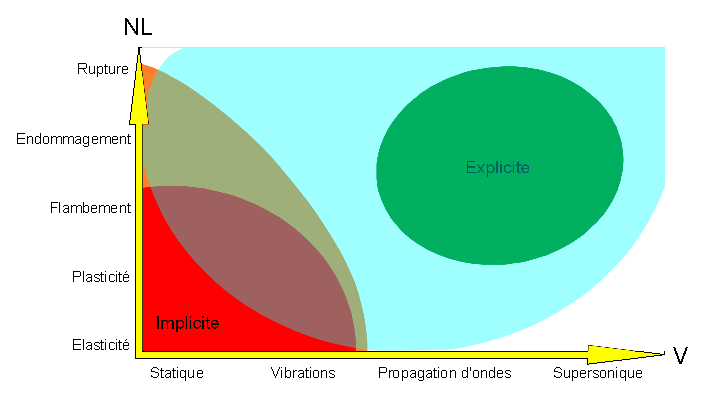
\includegraphics[height=80mm]{Im-Ex-plicite.eps}
\caption{Domaines d'utilisation des méthodes implicite et explicite}\label{Fig-Im-Ex-plicite}
\end{figure}
La \fig{Fig-Im-Ex-plicite} donne, de manière imagée, les domaines d'utilisation des méthodes implicite et explicite.


\section{Exemple: un calcul de propagation avec \freefem}

\medskip
Quelque soit le logiciel utilisé\footnote{Lorsque l'on parle de codes éléments finis, on cite les grands noms du domaine... et ils correspondent à des codes extraordinairement puissants, mais souvent chers.

Or un certain nombre de codes éléments finis professionnels sont disponibles gratuitement (au téléchargement et à l'utilisation). Les deux plus connus sont \castem (anciennement castem) et \aster développés et maintenus par le CEA et par EDF respectivement.}, il y a toujours un grand nombre d'exemples traités fournis avec, sans compter le nombre d'ouvrages disponibles.

\medskip
Nous avons souhaité néanmoins présenter un listing (qui sera discuté oralement) correspondant à un calcul réalisé sous \freefem.

Ce logiciel gratuit vous permettra de faire vos calculs par éléments finis... mais c'est également un outil pédagogique sans équivalent: sa manipulation se fait en des termes proches de la formulation mathématique, et en cela, il est une passerelle parfaite entre la théorie et la pratique de codes plus «industriels».

Le fait de pouvoir discrétiser à loisir une formulation variationnelle que l'on rentre soi-même est également un argument qui nous semble un vrai plus, même si cela commence à exister dans des codes commerciaux (mais reste confidentiel).\footnote{Notons que pour ceux qui préfèrent, il existe aussi \textsc{Rheolef}, un environnement C++ pour le calcul par éléments finis, qui reste proche, dans sa philosophie, de ce que propose \freefem. Nous ne le connaissons pas assez pour fournir des exemples dans ce document.}

\medskip
Voici donc un petit listing sur lequel nous pourrons revenir de vive voix.

Commençons donc, comme il se doit, par définir la géométrie du problème, paramétrée par~$a$ et~$b$, que nous maillons:

\medskip
\color{gris}\scriptsize
%\begin{multicols}{2}
\begin{Verbatim}[numbers=left,numbersep=3pt]
real mu=1.; 
real rog=0. , ro=1.;
// taille du maillage
int ncuts = 20;

// construction du domaine
real a=pi*0.8, b=1.2*pi ; 

border gam1(t=0.,a){x=t;y=0; label =1;};
border gam2(t=0.,b){x=a;y=t; label =2;};
border gam3(t=a,0.){x=t;y=b; label =3;};
border gam4(t=b,0.){x=0.;y=t; label =4;};

//Maillage
mesh Th=buildmesh(gam1(ncuts)+gam2(ncuts)+gam3(ncuts)+gam4(ncuts)); 
//plot(Th, ps="mesh.eps") ;
//plot(Th, wait=1) ;
\end{Verbatim}
%\end{multicols}
\color{black}\normalsize

\medskip
Nous définissons quelques valeurs afin de pouvoir définir le chargement (le chargement défini par la fonction~$w_1$ ne sera pas utilisée dans le calcul effectué). Notons comme il est aisé de définir des fonctions:

\color{gris}\scriptsize
\begin{multicols}{2}
\begin{Verbatim}[numbers=left,numbersep=3pt,firstnumber=last]
// conditions aux limites essentielles 
real r0=a/10., r, xc=a/3., yc=3.*b/4.; 

// chargement initial sinusoidal
func real pertb(real r)
	{ if(r<r0) {return (1.+cos(pi*r/r0));}
	else return 0.;}

//func real w1( real x, real y)
func real w11( real x, real y)
{
	return pertb(sqrt((x-xc)^2+(y-yc)^2)); 
}

// chargement constant sur un carre
// pas utilise sur cet exemple
func real w1( real c, real d)
{
 if(c>(0.8*xc))
   {if (c<(1.2*xc)) 
    {if (d>(0.8*yc))
      {if (d<(1.2*yc)) {return 0.8;}
      else return 0.;}
    else return 0.;}
   else return 0.;}
	else return 0.;
}

func real w0( real x, real y)
{
	return 0.*sin(x)*sin(y) ; 
}
\end{Verbatim}
\end{multicols}
\color{black}\normalsize

\medskip
Ensuite, nous définissons l'espace des éléments finis utilisés, et les variables appartenant à ces espaces. L'analogie avec la «formulation mathématique» saute au yeux... et c'est pourquoi cet outil nous semble particulièrement intéressant sur le plan pédagogique.

\color{gris}\scriptsize
%\begin{multicols}{2}
\begin{Verbatim}[numbers=left,numbersep=3pt,firstnumber=last]
// Espaces elements finis 
fespace Vh(Th,P2); 
fespace Wh(Th,P1dc);

Vh w, wa, wd, wda, wdd, wdda, fi ; 
Wh sxz, syz ; 
\end{Verbatim}
%\end{multicols}
\color{black}\normalsize

\medskip
Il s'agit d'un exemple non stationnaire, nous allons donc faire une boucle sur le temps. Dans \freefem, nous entrons directement la formulation variationnelle du problème sous forme «mathématique»... le lien entre pratique des éléments finis et théorie est beaucoup plus clair. La boucle de temps est basée sur un schéma de Newmark implicite. Le temps «courant» est le temps~$t+\Delta_t$ et le temps précédent est le temps~$t$ pour rester cohérent avec les notations du chapitre~\ref{Ch-temps}.

Il s'agit d'un problème de déplacement hors plan, dont le champ inconnu est traditionnellement noté~$w$. Ainsi, dans le listing, \verb|w| représente~$q_{t+\Delta_t}$, \verb|wa|$\equiv q_t$, 
\verb|wd|$\equiv \dot{q}_{t+\Delta_t}$, \verb|wda|$\equiv \dot{q}_t$, 
\verb|wdd|$\equiv \ddot{q}_{t+\Delta_t}$ et \verb|wdda|$\equiv \ddot{q}_t$. \verb|fi|$\equiv\varphi$
est la fonction test. La formulation variationnelle, en n'indiçant pas le temps actuel et en utilisant l'indice~$a$ pour le pas de temps précédent ($a$ comme avant), est:
\begin{equation}
\begin{array}{rl}
\text{antiplane}(\dot{w},\varphi) = &
	\dint_{Th} \rho \dot{w} \varphi + 
		\frac{\Delta_t^2}4 \dint_{Th} \mu \left( \dfrac{\partial \dot{w}}{\partial x}\dfrac{\partial \varphi}{\partial x} +
		\dfrac{\partial \dot{w}}{\partial y}\dfrac{\partial \varphi}{\partial y}\right)\\[+3ex]
	& - 	\dfrac{\Delta_t}2 \dint_{Th} \rho_g \varphi 
	- \dint_{Th} \rho\left(\dot{w}_a+\frac{\Delta_t}2 \ddot{w}_a\right)\varphi \\[+3ex]
	& + \dfrac{\Delta_t}2 \dint_{Th} \mu \left( \dfrac{\partial w_a}{\partial x}\dfrac{\partial \varphi}{\partial x}
		+ \dfrac{\partial w_a}{\partial y}\dfrac{\partial \varphi}{\partial y} \right) \\[+3ex]
	& + \dfrac{\Delta_t^2}4 \dint_{Th} \mu \left( \dfrac{\partial \dot{w}_a}{\partial x}\dfrac{\partial \varphi}{\partial x} +
		\dfrac{\partial \dot{w}_a}{\partial y}\dfrac{\partial \varphi}{\partial y} \right) \\[+3ex]
	& + \text{Condition } (\dot{w}=0 \text{ sur les lignes } 1,2,3,4)
\end{array}
\end{equation}

\color{gris}\scriptsize
%\begin{multicols}{2}
\begin{Verbatim}[numbers=left,numbersep=3pt,firstnumber=last]
int n, k, Ntemps=100; 
real T=2.*pi/sqrt(2.), pastemps=T/Ntemps
real dpt=0.5*pastemps; 

problem antiplane(wd,fi, init=1)=int2d(Th)(ro*wd*fi)+ 
		int2d(Th)(dpt^2*mu*(dx(wd)*dx(fi)+dy(wd)*dy(fi))) + 
		int2d(Th)(-dpt*rog*fi)+
		int2d(Th)(ro*(-wda-dpt*wdda)*fi)+
		int2d(Th)(dpt*mu*(dx(wa)*dx(fi)+dpt*dx(wda)*dx(fi)+
		dy(wa)*dy(fi)+dpt*dy(wda)*dy(fi)))+
		on(1,2,3,4,wd=0.); 

// formulation du probleme en temps
// conditions initiales en temps
w=w0(x,y);
wd=w11(x,y); 
wdd=0.; 

real errorw, errorwd, temps, enerC, enerP, enerT; 
real[int] visoS(20);
int ivi; 
for (ivi=0;ivi<10;ivi++){
	visoS[ivi]=-1+0.1*ivi;
	visoS[ivi+10]=(ivi+1)*0.1;
}
\end{Verbatim}
%\end{multicols}
\color{black}\normalsize

\medskip
Enfin, pour tester la qualité des résultats, il nous faut quelques indicateurs... Sans entrer dans le détail, des noms comme~\verb|enerC|, \verb|enerP|, et~\verb|enerT| doivent vous mettre sur la piste.

\color{gris}\scriptsize
%\begin{multicols}{2}
\begin{Verbatim}[numbers=left,numbersep=3pt,firstnumber=last]
real[int] Ec(Ntemps), Ep(Ntemps), Et(Ntemps), tt(Ntemps); 

for (n=0;n<Ntemps;n++){	
	wa=w; wda=wd; wdda=wdd; 	
	temps=n*pastemps; 

	enerC=0.5*int2d(Th)(ro*wd^2);
	enerP=0.5*int2d(Th)(mu*(dx(w)*dx(w)+ dy(w)*dy(w)));
	enerT=enerC+enerP;
	Ec(n)=enerC; Ep(n)=enerP; Et(n)=enerT; tt(n)=temps; 
		
	cout << " iteration n= " << n << " enerP= " << enerP << 
    "enerC= " << enerC << " enerTotale= " << enerT 
     << endl;
	
	temps=(n+1.)*pastemps; 

// resolution du probleme 
	antiplane;
	
	w=wa+dpt*(wda+wd);
	wdd=(wd-wda)/dpt-wdda; 

	sxz=mu*dx(w);
	syz=mu*dy(w); 
	plot(Th,wd,fill=true, value=1, viso=visoS, nbiso=visoS.n, 
     ps=n, wait=0); 	
}

// Energie 
//plot([tt,Ec], [tt,Ep],[tt,Et], ps="energie.eps"); 
\end{Verbatim}
%\end{multicols}
\color{black}\normalsize

\medskip
À la \fig{Fig-Exo6} se trouve une illustration de ce que nous venons de calculer.

\begin{figure}[h!]
  \center
  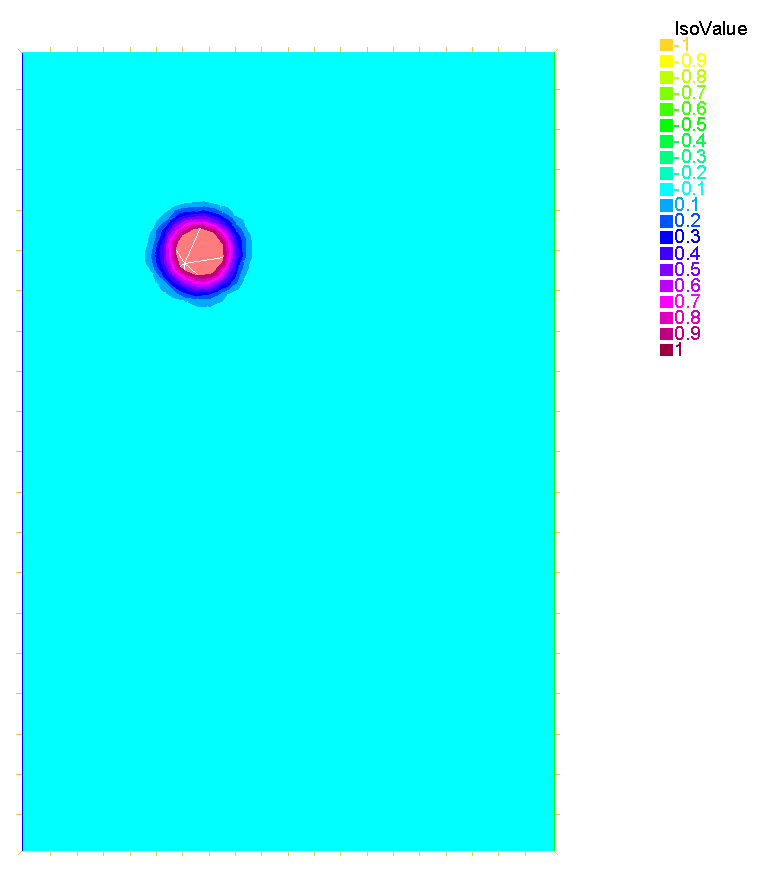
\includegraphics[height=55mm]{Exo6pas00.eps} \hfill
  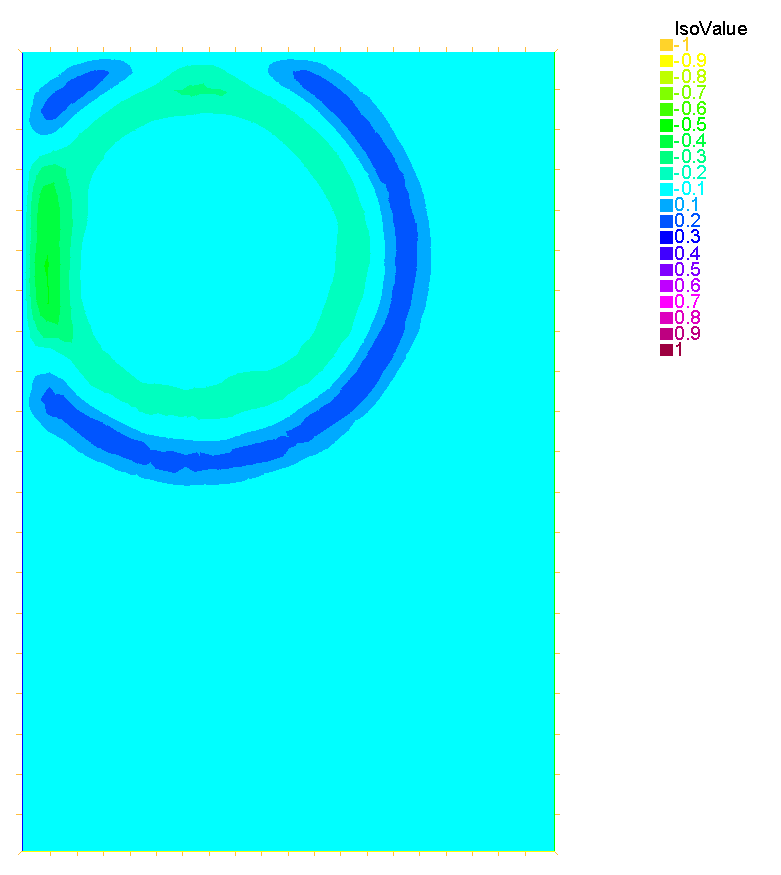
\includegraphics[height=55mm]{Exo6pas20.eps} \hfill
  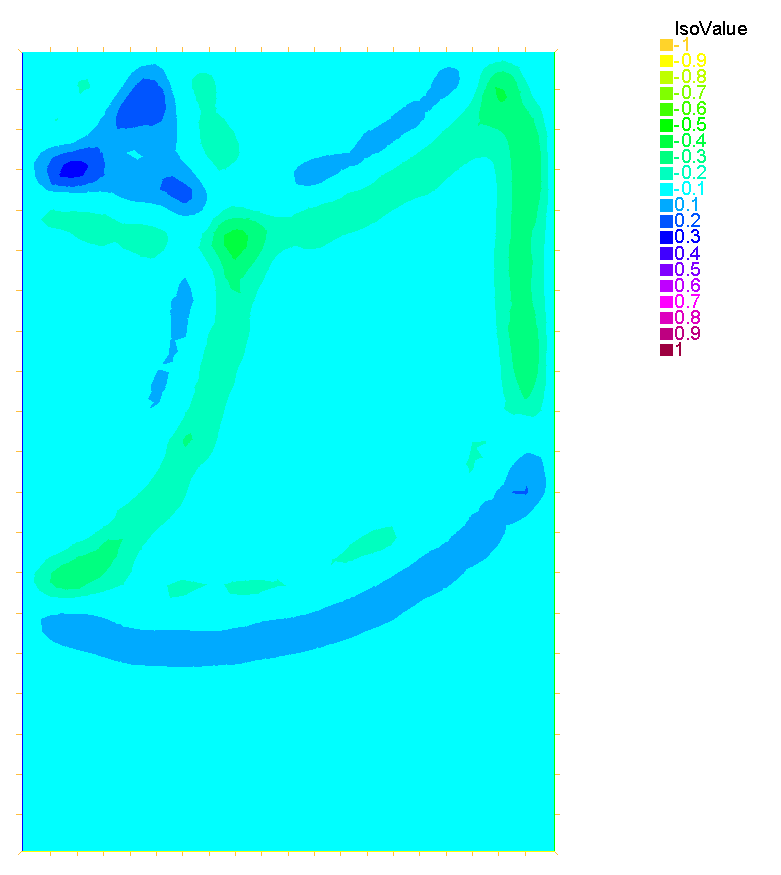
\includegraphics[height=55mm]{Exo6pas40.eps}
  \caption{\label{Fig-Exo6} Propagation: pas de temps 0, 20 et 40}
\end{figure}

% propagation freefem++


\bigskip
\section{Décomposition modale}\index{décomposition modale}

Pour le public visé, le lecteur devrait, à ce moment du document, se demander pourquoi il n'a pas encore été question de projection sur les modes propres.

\medskip
On peut montrer que les modes de vibration de la structure forment une base. Il peut paraître intéressant de chercher la solution en temps du problème sous forme d'une approximation par projection sur la base des quelques~$N$ premiers modes propres, i.e. de rechercher~$N$ fonctions scalaires du temps.

Lorsque l'on dispose déjà des~$N$ premiers modes et lorsque le nombre~$n$ de degrés de liberté est important, cette approche peut s'avérer particulièrement efficace. Par ailleurs, lorsque les modes sont associés à des mouvements simples de la structure, il peut être facile pour un ingénieur un peu expérimenté d'imaginer le nombre de modes à utiliser pour représenter le phénomène.

\medskip
La méthode de la décomposition modale sera exposée au paragraphe~\ref{Sec-RT}, lorsque nous aurons fait quelques rappels sur les modes propres.



%\medskip
%\section{La dynamique rapide}

%\medskip
%\subsection{Impact}

%\medskip
%\subsection{Crash}
